\documentclass[12pt, a4paper, simple]{eskdtext}

\usepackage{../_sty/title_variables}
\usepackage{../_sty/eskd_variables}
\usepackage{../_sty/sourceCode}
\usepackage{../_sty/tableOfContent}

% Графа 1 (наименование изделия/документа)
\ESKDcolumnI{\titlePageTopic\\Пояснительная записка}

% Графа 2 (обозначение документа)
\ESKDsignature{\code-\codePZ}

\begin{document}
    % Титульная страница
    \begin{ESKDtitlePage}
        \begin{center}
    МИНИСТЕРСТВО ОБРАЗОВАНИЯ РЕСПУБЛИКИ БЕЛАРУСЬ
    
    \hspace{0pt}

    УЧРЕЖДЕНИЕ ОБРАЗОВАНИЯ

    <<БРЕСТСКИЙ ГОСУДАРСТВЕННЫЙ ТЕХНИЧЕСКИЙ УНИВЕРСИТЕТ>>

    \hspace{0pt}

    КАФЕДРА \titlePageKafedra
\end{center}

\vfill

\begin{center}
    \titlePageTopic

    \hspace{0pt}

    ПОЯСНИТЕЛЬНАЯ ЗАПИСКА К КУРСОВОЙ РАБОТЕ

    ПО ДИСЦИПЛИНЕ <<\titlePageDistiplina>>
\end{center}

\vfill

\begin{center}
    \code-\codePZ

    \hspace{0pt}

    Листов \pageref{LastPage}
\end{center}

\vfill

\begin{flushright}
    \begin{minipage}[t]{.49\textwidth}
        \begin{minipage}[t]{.75\textwidth}
            \begin{flushright}
                Руководитель

                Выполнил

                Консультант

                по ЕСПД
            \end{flushright}
        \end{minipage}
    \end{minipage}
    \begin{minipage}[t]{.49\textwidth}
        \begin{flushright}
            \begin{minipage}[t]{.75\textwidth}
                \titlePageLeaderName~\titlePageLeaderSurname

                \titlePageAuthorName~\titlePageAuthorSurname

                \hspace{0pt}

                \titlePageConsultantName~\titlePageConsultantSurname

            \end{minipage}
        \end{flushright}
        
    \end{minipage}
\end{flushright}

\vfill

\begin{center}
    \ESKDtheYear
\end{center}
    \end{ESKDtitlePage}
    % Содержание
    \tableofcontents 
    \newpage
    % Введение
    \section*{ВВЕДЕНИЕ} % Секция без номера
\phantomsection
\addcontentsline{toc}{section}{ВВЕДЕНИЕ} % Добавить в содержание

В современном мире программисту приходится сталкиваться с огромным количеством информации, которую необходимо сохранить. Хранение информации – это ее запись во вспомогательные запоминающие устройства на различных носителях для последующего использования. Хранение является одной из основных операций, осуществляемых над информацией, и главным способом обеспечения ее доступности в течение определенного промежутка времени.

Данная курсовая работа предполагает решение следующих задач:

\begin{enumerate}
    \item Изучить, что такое информационные системы, принципы их создания и работы, объяснить их необходимость в жизни человека и описать сферы применения информационной системы <<Товары>>
    \item Изучить возможности и характеристики при создании приложения для работы с информационной системой <<Товары>>
    \item Спроектировать систему и создать приложение с данными на тему <<Товары>>.
\end{enumerate}

Информационная система (ИС) — система, предназначенная для хранения, поиска и обработки информации, и соответствующие организационные ресурсы (человеческие, технические, финансовые и т. д.), которые обеспечивают и распространяют информацию.

ИС предназначена для своевременного обеспечения надлежащих людей надлежащей информацией, то есть для удовлетворения конкретных информационных потребностей в рамках определённой предметной области, при этом результатом функционирования информационных систем является информационная продукция — документы, информационные массивы, базы данных и информационные услуги.

Первоначально для хранения информации на ЭВМ применялись локальные массивы (или файлы), при этом для каждой из решаемых функциональных задач создавались собственные файлы исходной и результатной информации. Это приводило к значительному дублированию данных, за счёт чего использовалось больше памяти вычислительной машины, а также усложнялось обновление хранимой информации.

С целью решения вышеописанных проблем были созданы своего рода электронные хранилища данных - базы данных. Базы данных - это часть информационных систем.

База данных представляет собой определенным образом структурированную совокупность данных, совместно хранящихся и обрабатывающихся в соответствии с некоторыми правилами. Как правило, БД моделирует некоторую предметную область или ее фрагмент. Очень часто в качестве постоянного хранилища информации баз данных выступают файлы.

Немаловажной является и взаимосвязь информации в базе данных: изменение одной строчки может привести к значительным изменениям других строк. Работать с данными таким образом гораздо проще и быстрее, чем если бы изменения касались только одного места в базе данных.

Помимо основной функции - хранения и систематизации огромного количества информации - они позволяют быстро обрабатывать клиентские запросы и выдавать актуальную информацию.

На сегодняшний день базы данных занимают одно из первых мест для многих организаций, которые для упрощения своей работы применяют компьютерные технологии.

Результатом разрабатываемой программы должно являться приложение, позволяющее пользователю взаимодействовать с данными о спортсменах футбольной команды при помощи пользовательского интерфейса.

\newpage
 
    % 1. Постановка задачи
    \newpage
\section{Постановка задачи}
\subsection{Перечень функций}

Достижение цели курсовой работы предполагает необходимость создания приложения для работы с локальной базой данных на тему <<Товары>> с использованием пользовательского интерфейса и решения следующих конкретных задач:

\begin{enumerate}
    \item [1.] Чтение и запись информации в базе данных.
    \item [2.] Удаление и обновление информации в базе данных.
    \item [3.] Сортировка записей в базе данных.
    \item [4.] Поиск по записям в базе данных.
\end{enumerate}
\subsection{Требования пользователей}

Пользовательские требования - описание на естественном языке (плюс поясняющие диаграммы) функций, выполняемых системой, и ограничений, накладываемых на неё.

Источники: Пользователь

Документ: Пользовательские требования/Требования к ПО

Ответственный: Системный аналитик

Эти требования должны определять только внешнее поведение системы, избегая по возможности определения структурных характеристик системы. Пользовательские требования должны быть написаны естественным языком с использованием простых таблиц, а также наглядных и понятных диаграмм.

Требования пользователя к информационной системе <<Товары>>:

Обязательные:

\begin{enumerate}
    \item [1.] Должна быть реализована функция ввода данных в информационную систему
    \item [2.] Должна работать функция удаления записи из информационной системы
    \item [3.] Информационная система должна осуществлять сортировку записей по одному или нескольким полям
    \item [4.] Информационная система должна осуществлять поиск по записям.
\end{enumerate}

Желательные:

\begin{enumerate}
    \item [1.] Информационная система должна выводить отчеты на печать.
\end{enumerate}
\subsection{Проектирование архитектуры ПО (модули)}

Архитектура программного обеспечения (англ. software architecture) - совокупность важнейших решений об организации программной системы.

Архитектура включает:

\begin{itemize}
    \item выбор структурных элементов и их интерфейсов, с помощью которых составлена система, а также их поведения в рамках сотрудничества структурных элементов
    \item соединение выбранных элементов структуры и поведения во всё более крупные системы
    \item архитектурный стиль, который направляет всю организацию - все элементы, их интерфейсы, их сотрудничество и их соединение.
\end{itemize}

Документирование архитектуры программного обеспечения (ПО) упрощает процесс коммуникации между разработчиками, позволяет зафиксировать принятые проектные решения и предоставить информацию о них эксплуатационному персоналу системы, повторно использовать компоненты и шаблоны проекта в других.

Архитектурный вид состоит из 2 компонентов:

\begin{enumerate}
    \item [1.] Элементы
    \item [2.] Отношения между элементами
\end{enumerate}

Архитектурные виды можно поделить на 3 основных типа:

\begin{itemize}
    \item [1.] Модульные виды (англ. module views) - показывают систему как структуру из различных программных блоков.
    \item [2.] Компоненты-и-коннекторы (англ. component-and-connector views) - показывают систему как структуру из параллельно запущенных элементов (компонентов) и способов их взаимодействия (коннекторов).
    \item [3.] Размещение (англ. allocation views) - показывает размещение элементов системы во внешних средах.
\end{itemize}

Примеры модульных видов:

Декомпозиция (англ. decomposition view) - состоит из модулей в контексте отношения <<является подмодулем>>.

Использование (англ. uses view) - состоит из модулей в контексте отношения <<использует>> (т.е. один модуль использует сервисы другого модуля).

Вид уровней (англ. layered view) - показывает структуру, в которой связанные по функциональности модули объединены в группы (уровни).

Вид классов/обобщений (англ. class/generalization view) - состоит из классов, связанные через отношения <<наследуется от>> и <<является экземпляром>>.

\subsubsection*{Иерархия модулей и подмодулей разрабатываемой программы}

Информационная система <<Товары>> включает в себя следующие модули:

\begin{itemize}
    \item Модуль организации локальной базы данных с выводом информации о товарах, включающий в себя меню
    \item Модуль, реализующий добавление новых записей в базу данных
    \item Модуль, осуществляющий сортировку записей в базе данных
    \item Модуль удаления записи/записей из локальной базы данных
    \item Модуль, осуществляющий поиск записи по реализованной базе данных
\end{itemize}

Некоторые модули являются подмодулями других, более общих модулей. Таким образом, в данной программе модули добавления, удаления, сортировки и поиска записи/записей будут являться подмодулями главного модуля, отвечающего за вывод локальной базы данных на экран с данными о спортсменах футбольной команды и организацией меню. Графически связь основного модуля с его подмодулями изображена на рисунке \ref{fig:modules} (рис. \pageref{fig:modules}).

\begin{figure}[!htp]
    \centering{
        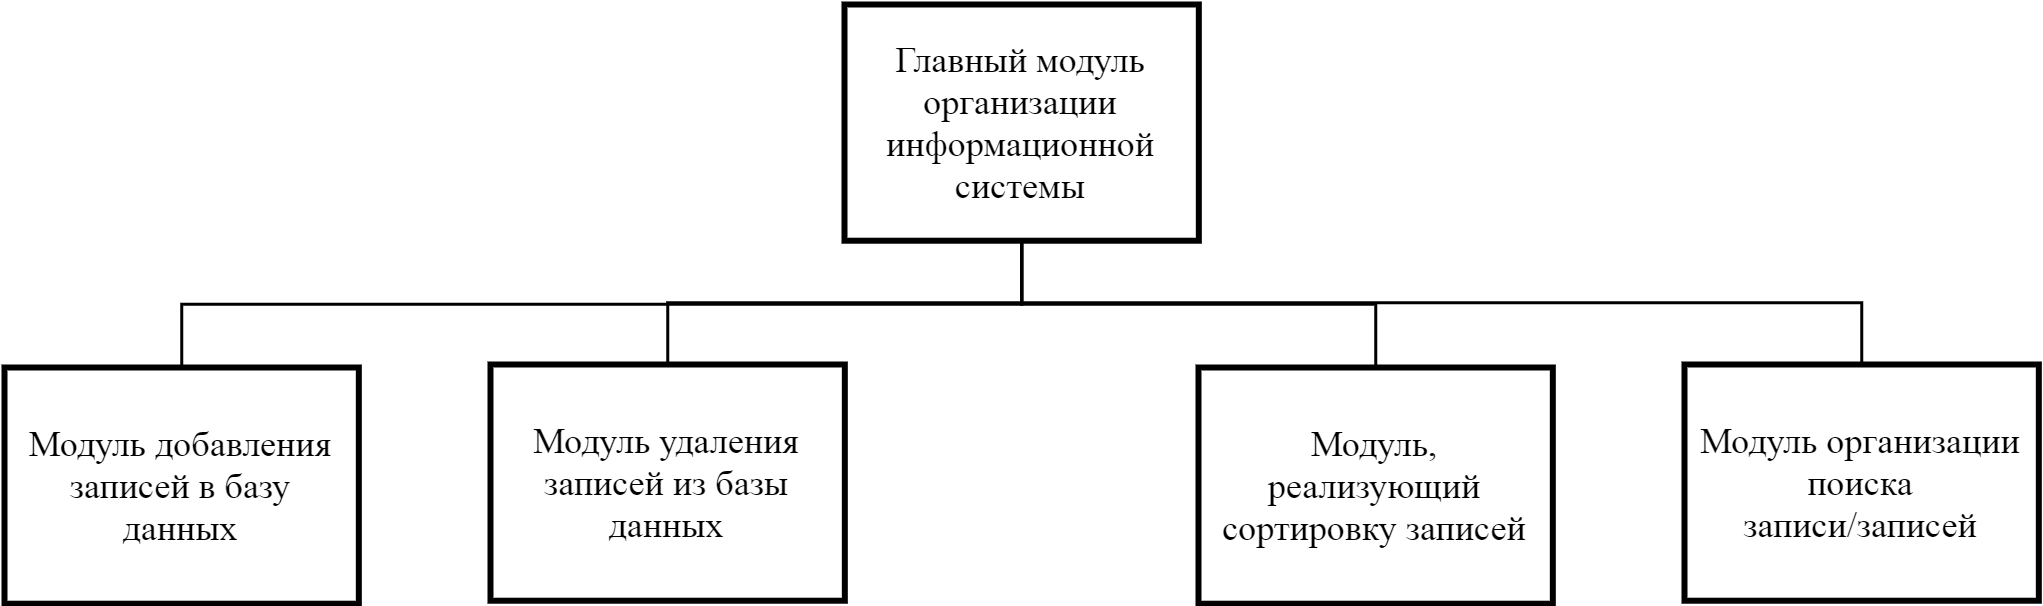
\includegraphics[]{_input/formulationOfTheProblem/softwareArchitectureDesignModules/modules.png}
    }
    \caption{Модули и подмодули}
    \label{fig:modules}
\end{figure}

\subsection{Проект. Схема данных}

Трёхуровневая архитектура - архитектурная модель программного комплекса, предполагающая наличие в нём трёх компонентов: клиента, сервера приложений (к которому подключено клиентское приложение) и сервера баз данных.

Если мы посмотрим на данную архитектуру с позиции сайта. То первый уровень можно считать браузером, с помощью которого посетитель заходит на сайт, второй уровень - это связка Apache2 + PHP, а третий уровень - это база данных MySQL.

\begin{figure}[!htp]
    \centering{
        
\includegraphics[]
        {../_input/formulationOfTheProblem/theProjectDataSchemas/softwareArchitectureDiagram.png}
    }
    \caption{Схема архитектуры ПО}
    \label{fig:layoyt}
\end{figure}

\subsection{Проектирование UI (макеты)}

Интерфейс будет содержать шапку сайта, которая в себе содержит навигацию (основный страницы).

В теле сайта на главной странице будет находится информация о том как начать пользоваться сайтом.

В теле сайта на странице добавления будет находится форма, через которую можно добавить поля в базу данных.

В теле сайта на странице вывода таблицы будет находится таблица с настройками поиска и сортировки, затем таблица с элементами из базы данных, которые отсортированы и отобраны по типу. Макет изображен на рисунке \ref{fig:layoyt} (стр. \pageref{fig:layoyt}).

\begin{figure}[!htp]
    \centering{
        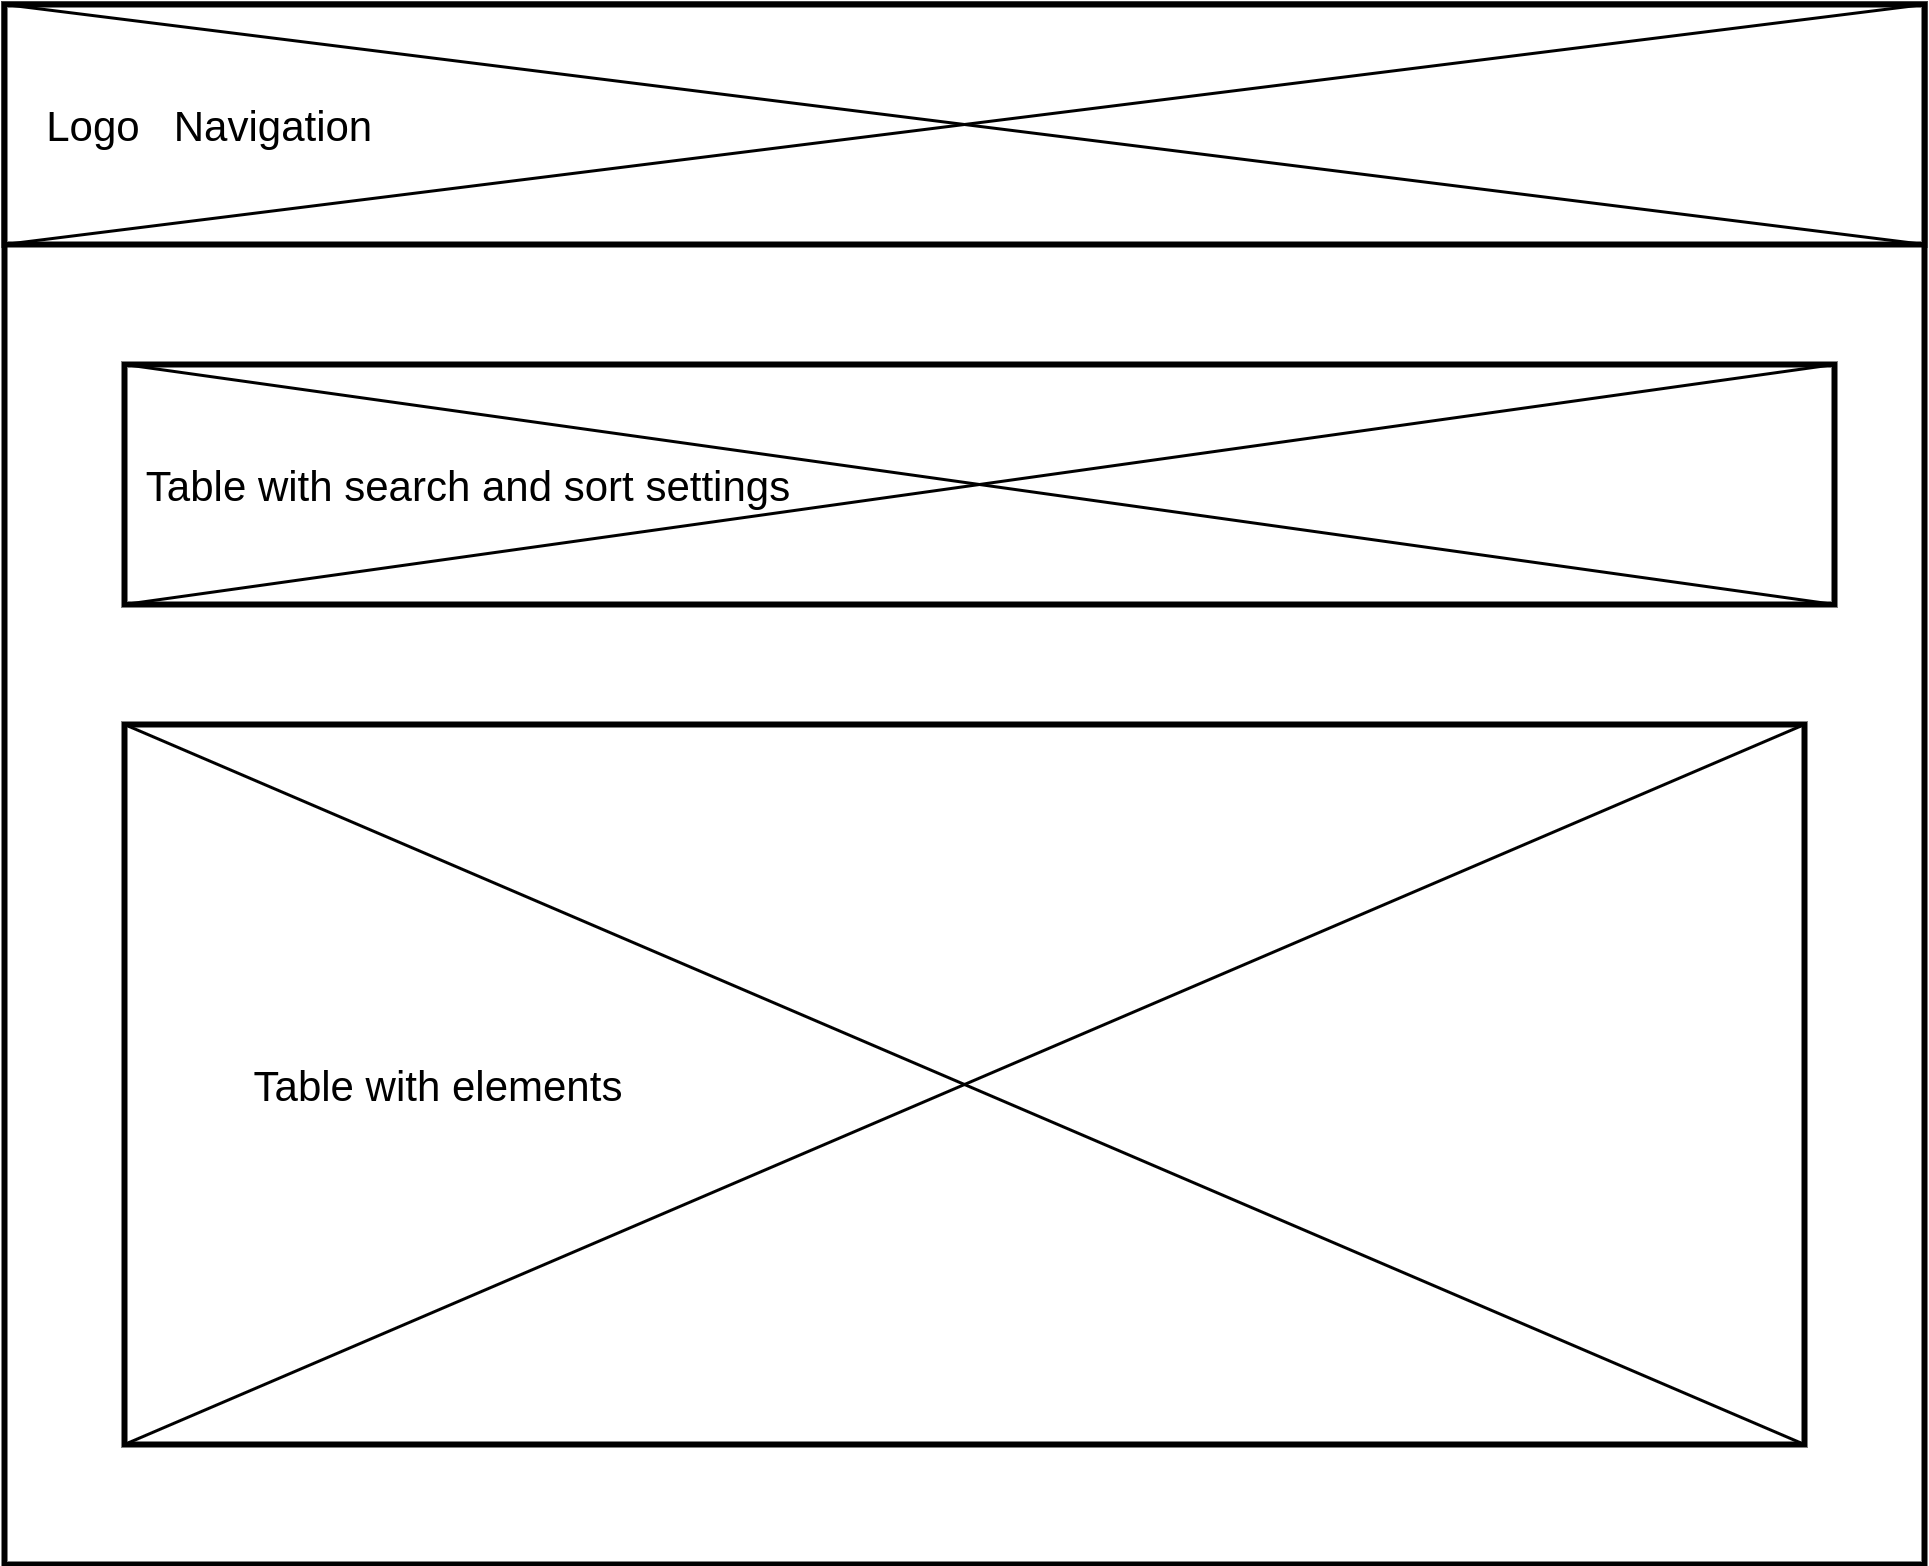
\includegraphics[width=15cm]
        {_input/formulationOfTheProblem/projectUI/layout.png}
    }
    \caption{Макет страницы}
    \label{fig:layoyt}
\end{figure}
\newpage 
    % 2. Разработка алгоритмов
    % 3. Разработка программы
    % 4. Тестирование программы
    \section{Тестирование программы}
        % Описание условий тестирования
        \subsection{Описание условий тестирования}

Данный проект разработан на PHP. Проект является сайтом. А значит его можно открыть в браузере.

\textbf{Использованный браузер для тестирования}: Mozilla Firefox 78.4.1esr (64-bit)

Сайт может открываться как на мобильных устройствах, так и на компьютере.

\textbf{Использованное устройство для тестирования}: компьютер с расширением экрана 1440x900.
        % Проверка всех функций реализованного ПО
        \subsection{Проверка функций реализованного ПО}
        \textbf{Тест}: <<Добавление полей в таблицу MySQL через форму на сайте>>

\underline{Ожидаемый результат}:
В таблицу MySQL добавяться поля через форму на сайте как элемент под определённым ID.

\underline{Описание}:
Тестирование правильности записи полей из формы
на рисунке \ref{fig:site_form}
(стр. \pageref{fig:site_form})
о добавления полей в таблицу MySQL.

\begin{figure}[!htp]
    \begin{center}
        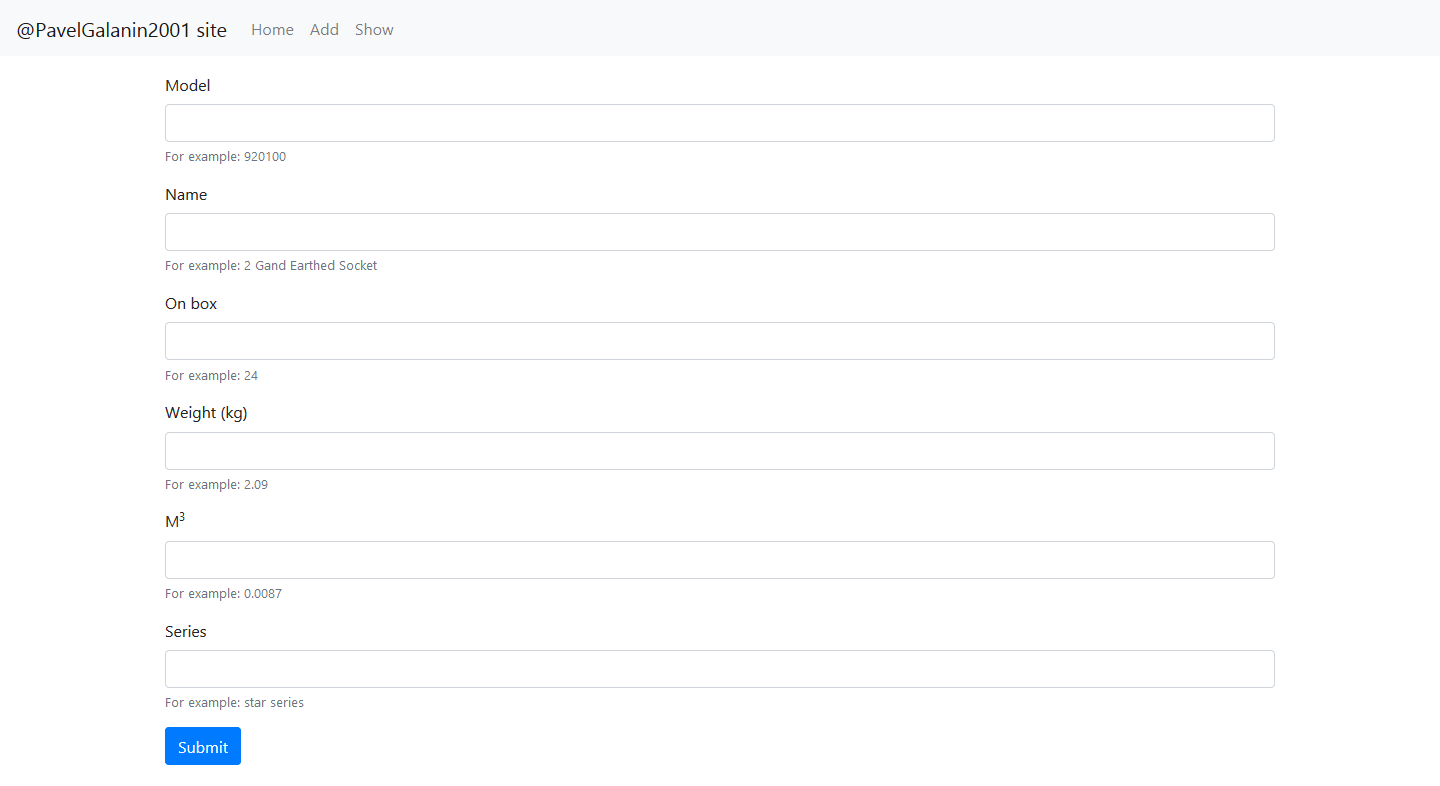
\includegraphics[width=12cm]{../_input/tests/site_form.png}
    \end{center}
    \caption{Форма для добавления элемента\label{fig:site_form}}
\end{figure}

\underline{Полученный результат}:

\begin{itemize}
    \item Таблица MySQL до добавления элемента
    на рисунке \ref{fig:mysql_table_before}
    (стр. \pageref{fig:mysql_table_before}).

    \item Вывод таблицы на сайте до добавления элемента
    на рисунке \ref{fig:site_table_before}
    (стр. \pageref{fig:site_table_before}).

    \item Форма на сайте с заполеными полями
    на рисунке \ref{fig:site_form_add_element_to_table}
    (стр. \pageref{fig:site_form_add_element_to_table}).

    \item Таблица MySQL после добавления элемента
    на рисунке \ref{fig:mysql_table_after}
    (стр. \pageref{fig:mysql_table_after}).

    \item Вывод таблицы на сайте после добавления элемента
    на рисунке \ref{fig:site_table_after}
    (стр. \pageref{fig:site_table_after}).
\end{itemize}

\begin{figure}[!htp]
    \begin{center}
        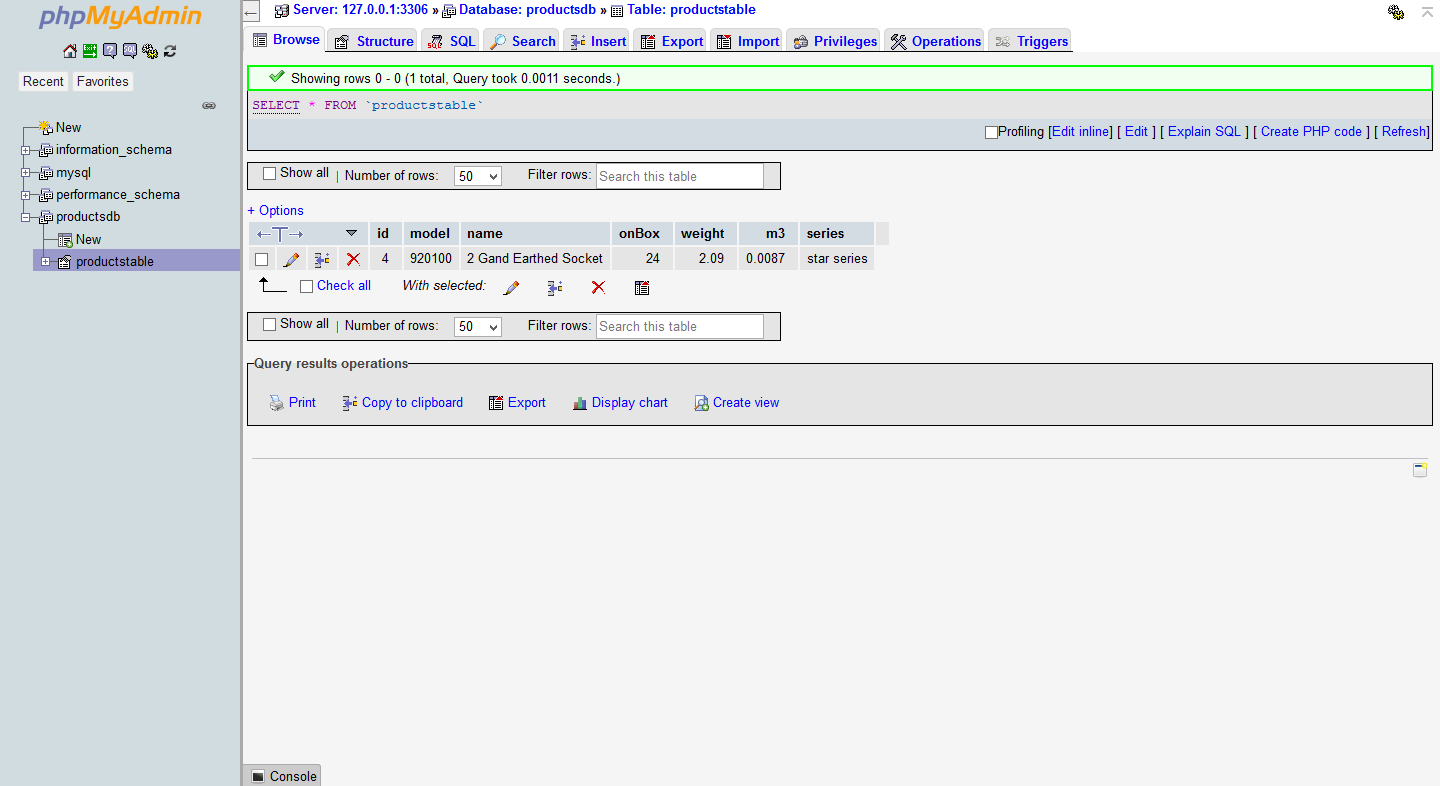
\includegraphics[width=12cm]{../_input/tests/mysql_table_before.png}
    \end{center}
    \caption{Таблица MySQL до добавления элемента\label{fig:mysql_table_before}}
\end{figure}

\begin{figure}[!htp]
    \begin{center}
        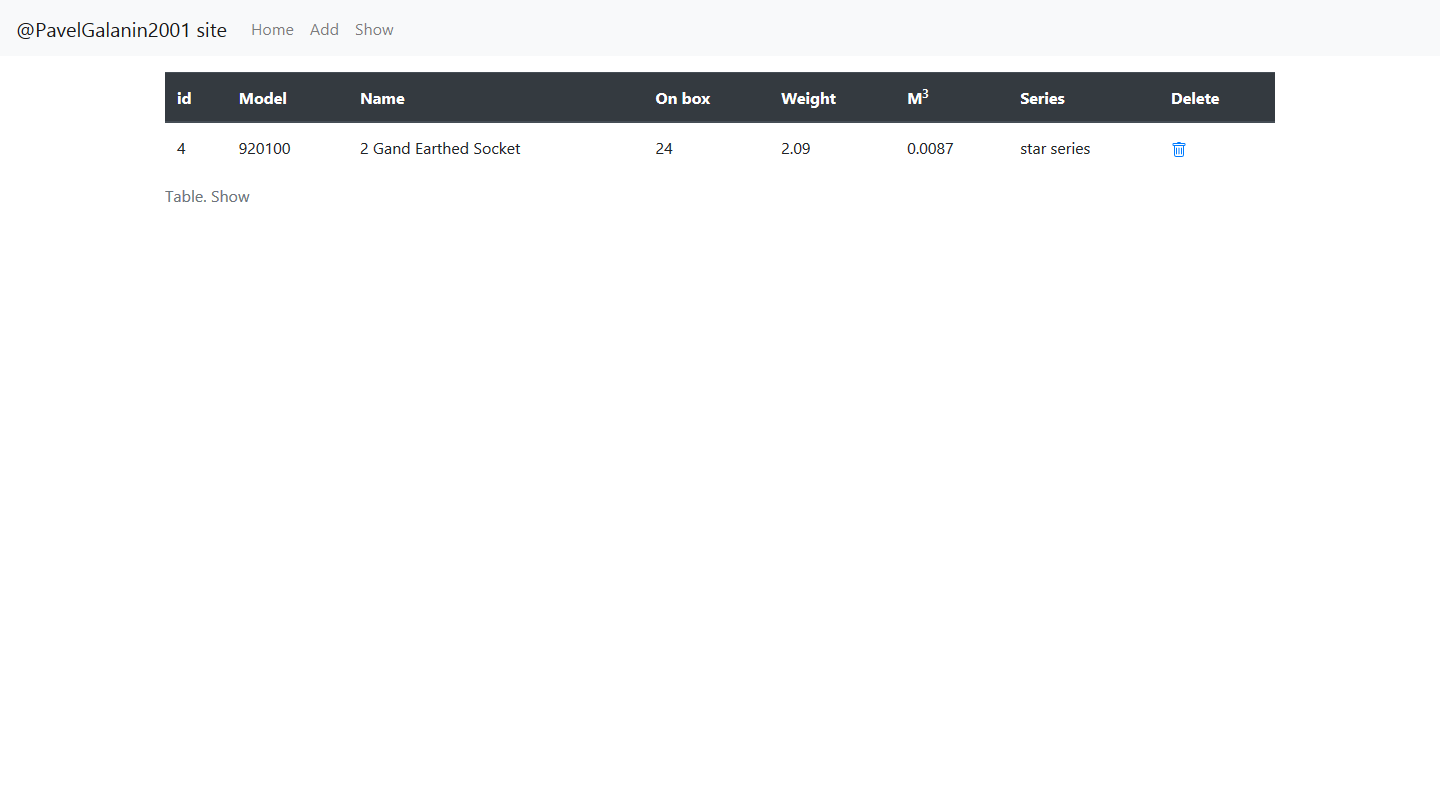
\includegraphics[width=12cm]{../_input/tests/site_table_before.png}
    \end{center}
    \caption{Вывод таблицы на сайте до добавления элемента\label{fig:site_table_before}}
\end{figure}

\begin{figure}[!htp]
    \begin{center}
        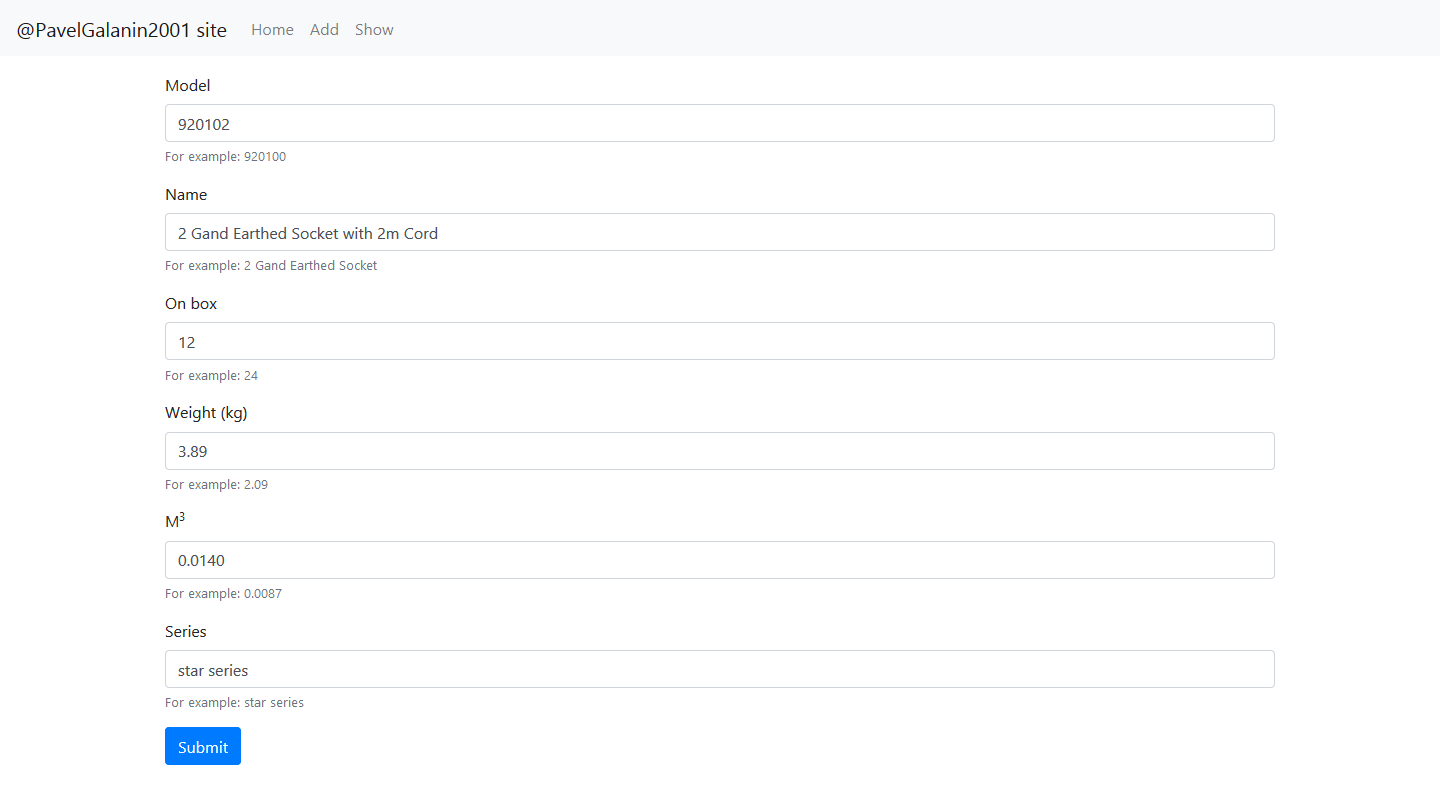
\includegraphics[width=12cm]{../_input/tests/site_form_add_element_to_table.png}
    \end{center}
    \caption{Форма на сайте с заполеными полями\label{fig:site_form_add_element_to_table}}
\end{figure}


\begin{figure}[!htp]
    \begin{center}
        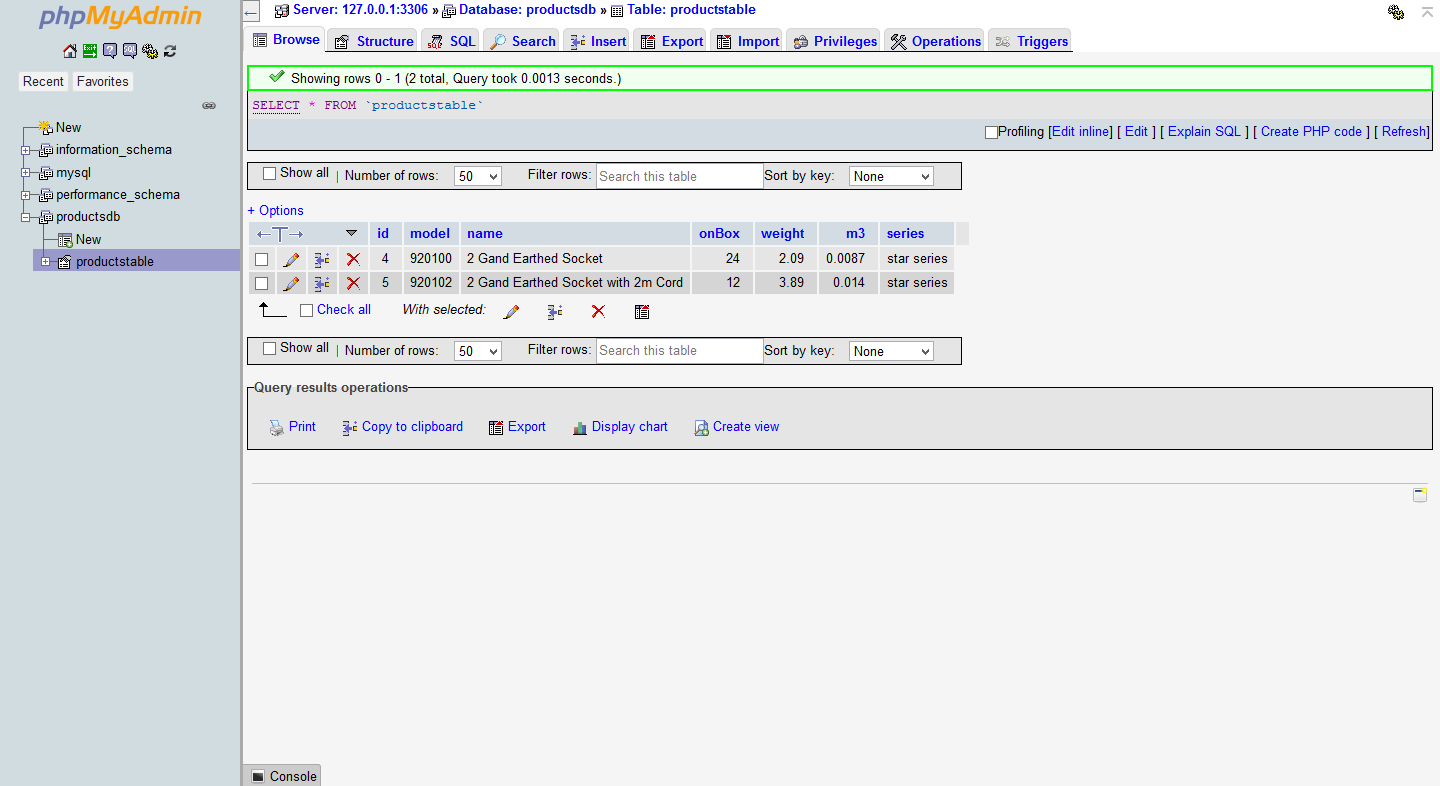
\includegraphics[width=12cm]{../_input/tests/mysql_table_after.png}
    \end{center}
    \caption{Таблица MySQL после добавления элемента\label{fig:mysql_table_after}}
\end{figure}

\begin{figure}[!htp]
    \begin{center}
        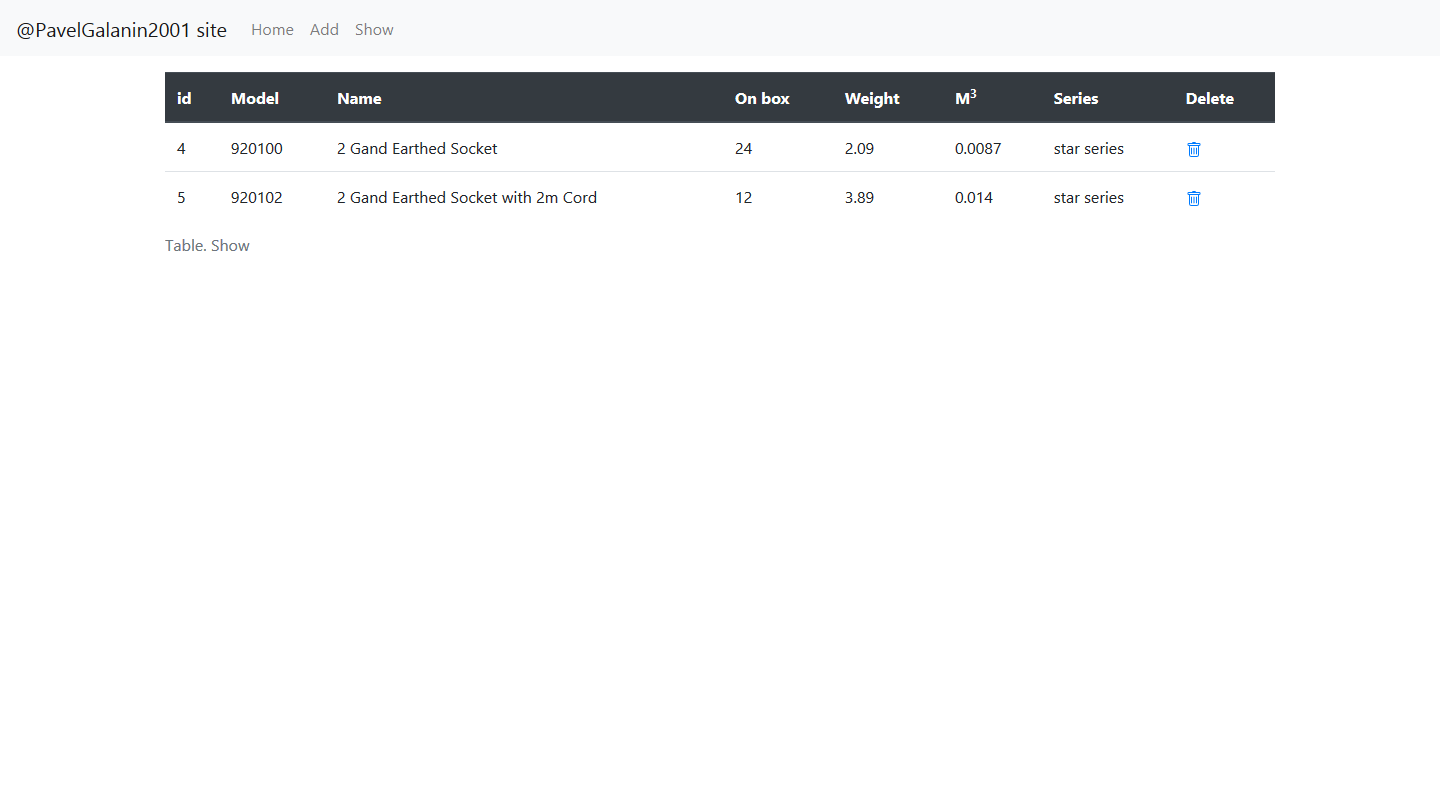
\includegraphics[width=12cm]{../_input/tests/site_table_after.png}
    \end{center}
    \caption{Вывод таблицы на сайте после добавления элемента\label{fig:site_table_after}}
\end{figure}

\underline{Вывод}:
Добавление полей в таблицу MySQL через форму на сайте работает корректно. Поля добавились в таблицу под определённым ID. Ожидаемый результат совпал с полученым.

        \newpage
        \textbf{Тест}: <<Удаление элемента из таблицы MySQL через таблицу на сайте>>

\underline{Ожидаемый результат}:
Из таблицы MySQL удалиться элемент, который был удален при нажатии иконки <<Корзина>> в таблице на сайте.

\underline{Описание}:
Тестирование правильности удаления элемента из таблицы MySQL через таблицу на сайте, по нажатию иконки <<корзина>>
на рисунке \ref{fig:test_delete_element__site_table}
(стр. \pageref{fig:test_delete_element__site_table})
о добавления полей в таблицу MySQL.

\begin{figure}[!htp]
    \begin{center}
        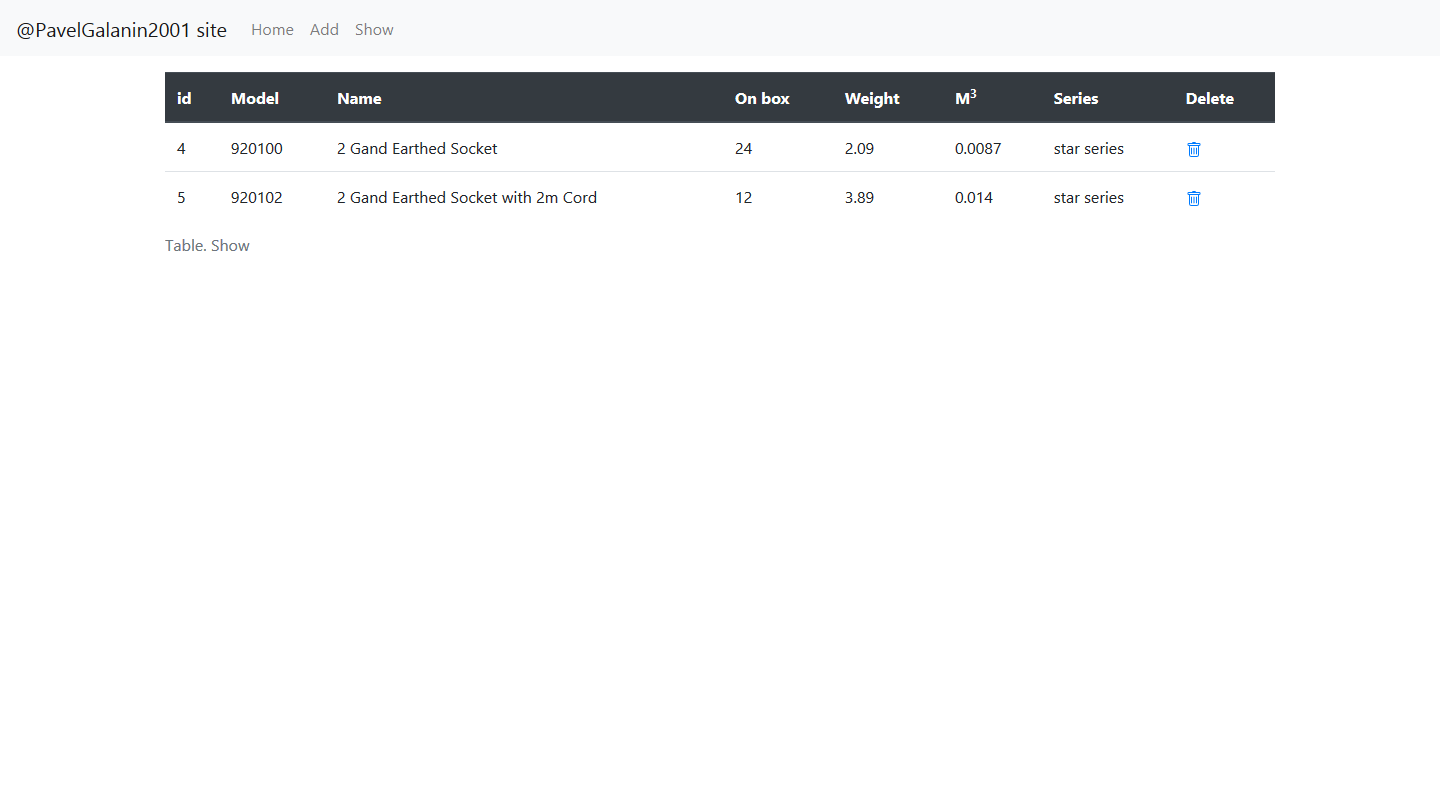
\includegraphics[width=12cm]{../_input/tests/site_table_after.png}
    \end{center}
    \caption{Форма для добавления элемента\label{fig:test_delete_element__site_table}}
\end{figure}

\underline{Полученный результат}:

\begin{itemize}
    \item Таблица MySQL после удаления элемента
    на рисунке \ref{fig:mysql_table_after_deleting}
    (стр. \pageref{fig:mysql_table_after_deleting}).

    \item Вывод таблицы на сайте после удаления элемента
    на рисунке \ref{fig:site_table_after_deleting}
    (стр. \pageref{fig:site_table_after_deleting}).
\end{itemize}

\begin{figure}[!htp]
    \begin{center}
        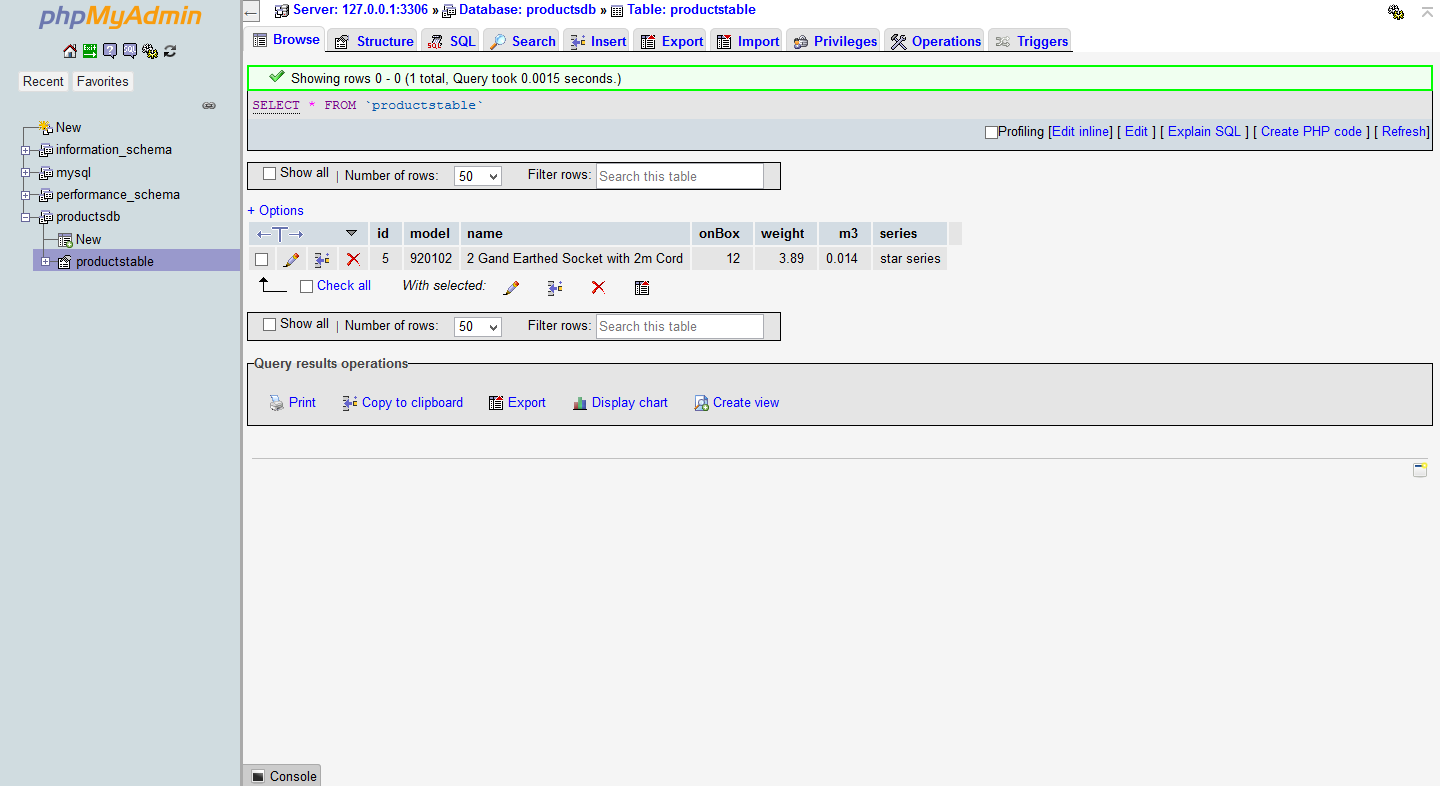
\includegraphics[width=12cm]{../_input/tests/mysql_table_after_deleting.png}
    \end{center}
    \caption{Таблица MySQL после удаления элемента\label{fig:mysql_table_after_deleting}}
\end{figure}

\begin{figure}[!htp]
    \begin{center}
        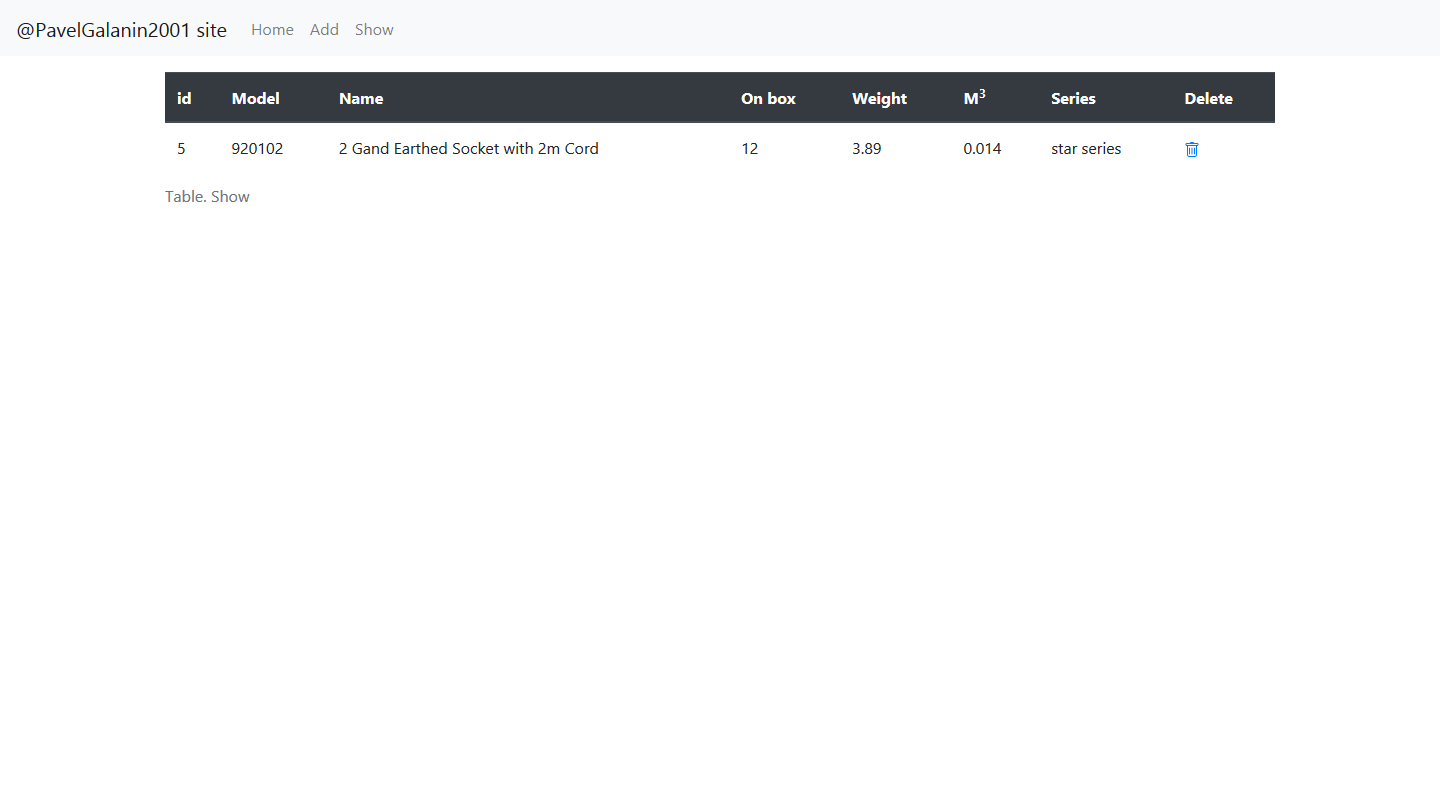
\includegraphics[width=12cm]{../_input/tests/site_table_after_deleting.png}
    \end{center}
    \caption{Вывод таблицы на сайте после удаления элемента\label{fig:site_table_after_deleting}}
\end{figure}

\underline{Вывод}:
Удаление элемента из таблицы MySQL через таблицу на сайте по кнопке <<корзина>> работает корректно. Элемент удалился из таблицы под определённым ID. Ожидаемый результат совпал с полученным.

    % Заключение
    % Список использованных источников
    % Приложение А. Текст программы
    % Приложение Б. Схема алгоритма
\end{document}